\documentclass[11pt,a4paper]{article}
\usepackage[margin=2.5cm]{geometry}
\usepackage[utf8]{inputenc}
\usepackage[T1]{fontenc}
\usepackage{hyperref}
\renewcommand{\familydefault}{\sfdefault}
\usepackage{helvet}
\pagestyle{empty}
\usepackage[kerning=true]{microtype}
\usepackage{parskip}
\usepackage{sansmath}
\usepackage[font={small, bf}]{caption}
\usepackage[font={small}]{subcaption}
\usepackage{graphicx}
\usepackage{multicol}
\setlength{\abovecaptionskip}{0pt}
\setlength{\floatsep}{10pt}
\setlength{\textfloatsep}{0pt}
\setlength{\intextsep}{0pt}
\setlength{\belowcaptionskip}{0pt}
\setlength{\parindent}{5ex}
\setlength{\parskip}{0pt}
% Feel free to use additional packages for glosses, figures, whatnot.

% The next bit is for reserving sufficient space for authors,
% affiliations, and e-mail address.  No need to change for initial
% anonymous version.  For the final version, replace the
% \toggletrue{anonymous} with \togglefalse{anonymous} to de-anonymize.
\usepackage{etoolbox}
\newtoggle{anonymous}
\togglefalse{anonymous}

\renewcommand{\title}[1]{\textbf{#1}\\}
\newcommand{\authors}[1]{\iftoggle{anonymous}{\phantom{#1}}{#1}\\}
\newcommand{\email}[1]{\iftoggle{anonymous}{\phantom{#1}}{#1}}

\begin{document}

% First page:

% Insert title, authors, affiliations, and e-mail address in the next three lines:

\title{TODO TITLE}
\authors{Veronica Boyce, Ilaria Chen, Bobby Sparks, Malia Perez, Michael C. Frank} 
\email{vboyce@stanford.edu;  Stanford University}
\newline
%

% Intro
%TODO citations

%TODO math

%TODO crossref figures!

As children acquire language, they must master many communication skills such as using metaphor and tracking the knowledge state of their partner. Adults demonstrate their communicative abilities in iterated reference games, where they describe novel figures to communicative partners with high accuracy. Over repetitions, description length reduces as partners come to share a nickname for the figure (Clark \& Wilkes-Gibbs 1986, Hawkins et al. 2020). This paradigm is commonly studied with adults, but very little research on iterated communication games has been done with pre-literate children. 

Glucksberg et al. (1966) found that 5 year old children were not able to successfully communicate with each other about novel figures in a more complicated paradigm involving stacking blocks. However, children as young as 4 were successful at a two-choice, child-friendly iterated reference game when playing with their parent (Leung et al., 2020). Here, we test child-child dyads using a simplified version of Leung et al. 2020 to determine if children can communicate with each other about novel figures and whether they show partner-specificity. 



\textbf{Methods:} Pairs of children played a matching game on tablets while sitting across the table from each other. On each trial, the "speaker" child would see two images, one in a box, and describe the boxed image (orally) to their partner. The "listener" child saw the same two images and was tasked with helping Smurfy (a stuffy) guess the matching target image by touching it on the screen. Children alternated roles trial by trial; to help children keep track of role, they passed Smurfy back and forth. We had 4 target images (a subset of stimuli from Leung et al. 2020); distractors were drawn from the set of other targets. Children completed 2 practice trials with familiar shapes, and then 12 target trials (3 blocks of the 4 target images). We recruited 4-5 year old children from a university preschool; 20 pairs completed at least 8 out of 12 target trials and were included in the analysis. Children's utterances were transcribed from video recording, using Whisper and hand-checked. 
% Results

\textbf{Results:} 
Children were above chance at selecting the target image, and accuracy barely increased over time ($\beta=$0.13 [-.04, .31]). Children's speed to selecting a target increased over time ($\beta=$-1.24 [-1.89, -.59]). Children generally produced short descriptions, and the length of descriptions tended to slightly increase over time ($\beta=$0.11 [-.03, .25]). 

To compare the similarities of children's descriptions to those of their partners and other children; we embedded the utterances using S-BERT (Reimers \& Gurevych 2019) and used pairwise cosine similarity of embeddings as a proxy for utterance similarity. Children's utterances for an image are most similar to their own descriptions of the same image in different blocks. However, children's descriptions for an image are more similar to their partner's descriptions than the descriptions of children in other games. This indicates some level of partner specificity -- children are not just talking past each other, but are influenced by what their partner has said. 

\textbf{Caveats and Future Directions:} 
Transcripts of the sessions revealed that the research assistant echoed the children's descriptions on the majority of trials (ex: "Mary says she sees a bear. Do you see a bear?"). While this does not add any description not given by the children, repetition and prosody could influence children, and it does lend some "authority" to the description. Additionally, we have a small sample size of only 20 pairs of children, 4 images, and 3 repetitions. In a planned experiment 2, we will replicate this experiment, with a clearer experimenter script to avoid echoing and additional tweaks to clarify the procedure. 

This preliminary study suggests that (contra Glucksberg et al.) 4-5 year old children *can* describe and select novel figures with each other at above chance accuracy. However, the initially short utterances and lack of reduction offers intriguing suggestions about possible differences between children's and adults approaches. These could be due to different linguistic abilities, social expectations, or different task difficulty. 
\newpage

\begin{figure}
%TODO open materials
	\caption{Schematic of methods}
 \begin{center}{ 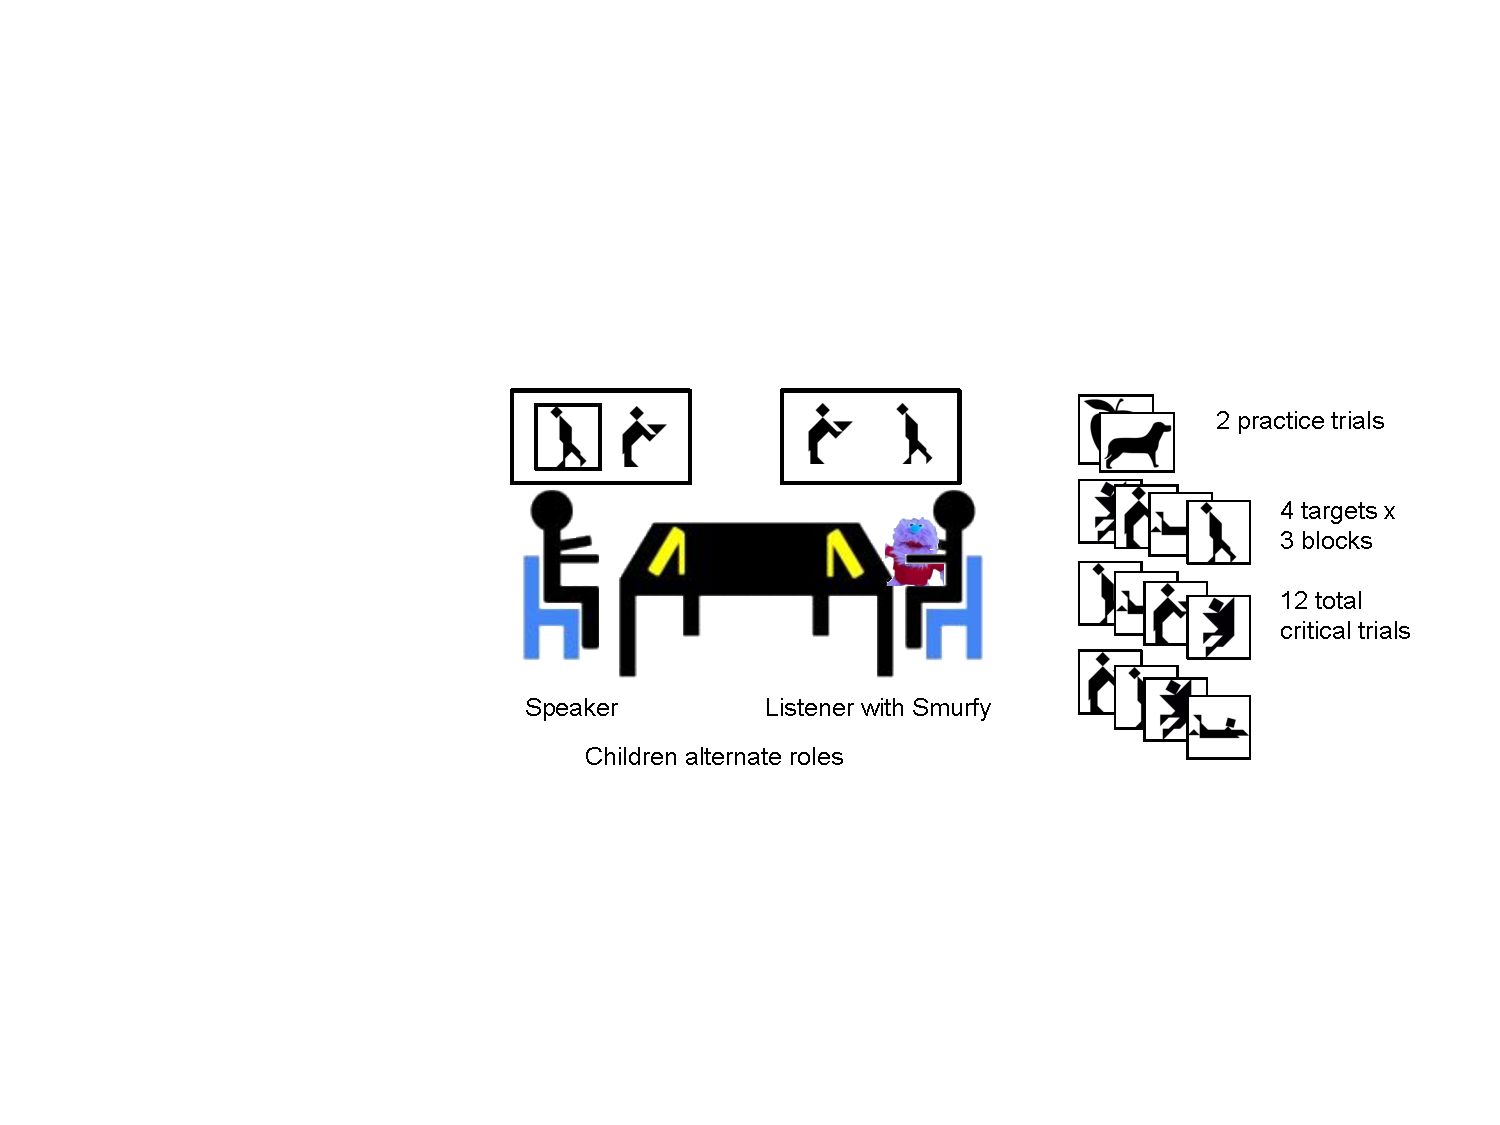
\includegraphics[width=.8\textwidth, trim={8cm 6cm 1cm 6.4cm}, clip]{exp-diagram.pdf}}
 	\end{center}
\end{figure}
	\begin{figure}
		\begin{minipage}{.5\textwidth}
			\captionof{figure}{Results}
			{	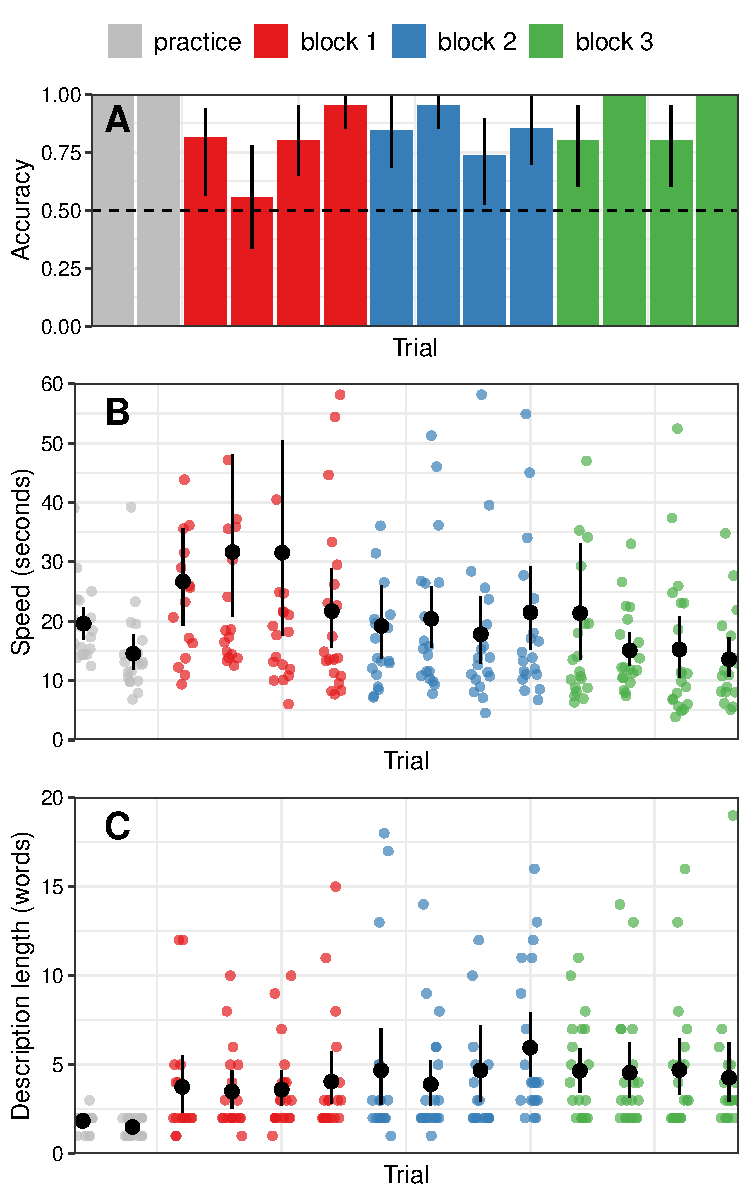
\includegraphics[width=\textwidth]{plot1.pdf}} 
			\begin{small}
			\textbf{	A.} Children's accuracy is at ceiling on practice trials and above chance on target trials.\textbf{ B.} Children speed up over time on target trials. \textbf{C.} Children's descriptions are usually short, but do not reduce in length over time. 
				
			\end{small}
			
		\end{minipage}
		~~~
		\begin{minipage}{.5\textwidth}	
		\captionof{figure}{Similarity Results}
		{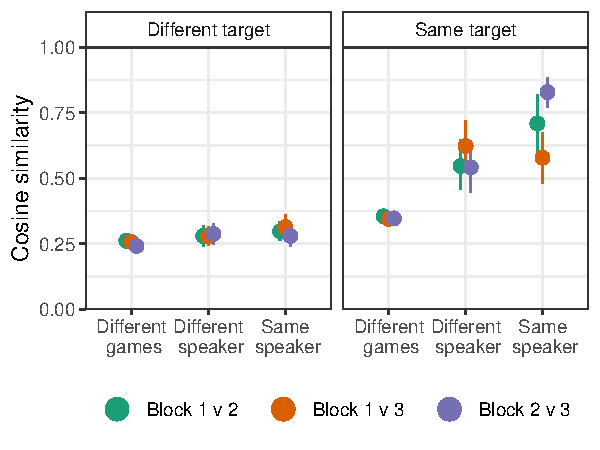
\includegraphics[width=\textwidth]{sims.pdf}} 
		\begin{small}
		Descriptions given by children were compared using sentence embeddings. Descriptions were most similar when provided by the same child for the same image. However, children described images more similarly to their partners than to children in other games.  Across games, the same image is described more similarly than different images.
		\end{small}
		
		\bigskip
		\begin{small}
\textbf{\centering Example successful descriptions:\\}
		a person $\bullet$ a person walking $\bullet$ sad walking $\bullet$ a man with two foot and a diamond shaped tummy and a square head
		
		a flying person $\bullet$
		a superhero$\bullet$
		somebody jumping $\bullet$ two wings with a square in the back with two feet
		
		someone building a funnel $\bullet$
		a server$\bullet$
		a person holding up a plate $\bullet$ a man with one foot and a line and a square and a triangle
		
		
		a crocodile tasting an animal in the water$\bullet$
		a whale$\bullet$
		someone flying a plane without a cover$\bullet$
		a person lying on the ground
		
		\end{small}
		\end{minipage}
	\end{figure}



\begin{figure}
	\begin{small} \textbf{References:}
Leung, Hawkins, Yurovsky. Cogsci, 2020. $\bullet$ Glucksberg, Krauss, Weisberg. J of Expt Child Psychology, 1966. $\bullet$ Clark \& Wilkes-Gibbs. Cognition, 1986. $\bullet$ Hawkins, Frank, Goodman. Cognitive Science, 2020. $\bullet$ Reimers \& Gurevych. arXiv 2019.
\end{small}
\end{figure}
\end{document}